\documentclass[12pt,twoside]{article}
\usepackage[dvipsnames]{xcolor}
\usepackage{tikz,graphicx,amsmath,amsfonts,amscd,amssymb,bm,cite,epsfig,epsf,url}
\usepackage[hang,flushmargin]{footmisc}
\usepackage[colorlinks=true,urlcolor=blue,citecolor=blue]{hyperref}
\usepackage{amsthm,multirow,wasysym,appendix}
\usepackage{array,subcaption} 
% \usepackage[small,bf]{caption}
\usepackage{bbm}
\usepackage{pgfplots}
\usetikzlibrary{spy}
\usepgfplotslibrary{external}
\usepgfplotslibrary{fillbetween}
\usetikzlibrary{arrows,automata}
\usepackage{thmtools}
\usepackage{blkarray} 
\usepackage{textcomp}
\usepackage[left=0.8in,right=1.0in,top=1.0in,bottom=1.0in]{geometry}

%% Probability operators and functions
%
% \def \P{\mathrm{P}}
\def \P{\mathrm{P}}
\def \E{\mathrm{E}}
\def \Var{\mathrm{Var}}
\let\var\Var
\def \Cov {\mathrm{Cov}} \let\cov\Cov
\def \MSE {\mathrm{MSE}} \let\mse\MSE
\def \sgn {\mathrm{sgn}}
\def \R {\mathbb{R}}
\def \C {\mathbb{C}}
\def \N {\mathbb{N}}
\def \Z {\mathbb{Z}}
\def \cV {\mathcal{V}}
\def \cS {\mathcal{S}}

\newcommand{\RR}{\ensuremath{\mathbb{R}}}

\DeclareMathOperator*{\argmin}{arg\,min}
\DeclareMathOperator*{\argmax}{arg\,max}
\newcommand{\red}[1]{\textcolor{red}{#1}}
\newcommand{\blue}[1]{\textcolor{blue}{#1}}
\newcommand{\green}[1]{\textcolor{ForestGreen}{ #1}}
\newcommand{\fuchsia}[1]{\textcolor{RoyalPurple}{ #1}}



%
%% Probability distributions
%
%\def \Bern    {\mathrm{Bern}}
%\def \Binom   {\mathrm{Binom}}
%\def \Exp     {\mathrm{Exp}}
%\def \Geom    {\mathrm{Geom}}
% \def \Norm    {\mathcal{N}}
%\def \Poisson {\mathrm{Poisson}}
%\def \Unif    {\mathrm {U}}
%
\DeclareMathOperator{\Norm}{\mathcal{N}}

\newcommand{\bdb}[1]{\textcolor{red}{#1}}

\newcommand{\ml}[1]{\mathcal{ #1 } }
\newcommand{\wh}[1]{\widehat{ #1 } }
\newcommand{\wt}[1]{\widetilde{ #1 } }
\newcommand{\conj}[1]{\overline{ #1 } }
\newcommand{\rnd}[1]{\tilde{ #1 } }
\newcommand{\rv}[1]{ \rnd{ #1}  }
\newcommand{\rM}{\rnd{ m}  }
\newcommand{\rx}{\rnd{ x}  }
\newcommand{\ry}{\rnd{ y}  }
\newcommand{\rz}{\rnd{ z}  }
\newcommand{\ra}{\rnd{ a}  }
\newcommand{\rb}{\rnd{ b}  }
\newcommand{\rt}{\rnd{ t}  }
\newcommand{\rs}{\rnd{ s}  }


\newcommand{\rpc}{\widetilde{ pc}  }
\newcommand{\rndvec}[1]{\vec{\rnd{#1}}}

\def \cnd {\, | \,}
\def \Id { I }
\def \J {\mathbf{1}\mathbf{1}^T}

\newcommand{\op}[1]{\operatorname{#1}}
\newcommand{\setdef}[2]{ := \keys{ #1 \; | \; #2 } }
\newcommand{\set}[2]{ \keys{ #1 \; | \; #2 } }
\newcommand{\sign}[1]{\op{sign}\left( #1 \right) }
\newcommand{\trace}[1]{\op{tr}\left( #1 \right) }
\newcommand{\tr}[1]{\op{tr}\left( #1 \right) }
\newcommand{\inv}[1]{\left( #1 \right)^{-1} }
\newcommand{\abs}[1]{\left| #1 \right|}
\newcommand{\sabs}[1]{| #1 |}
\newcommand{\keys}[1]{\left\{ #1 \right\}}
\newcommand{\sqbr}[1]{\left[ #1 \right]}
\newcommand{\sbrac}[1]{ ( #1 ) }
\newcommand{\brac}[1]{\left( #1 \right) }
\newcommand{\bbrac}[1]{\big( #1 \big) }
\newcommand{\Bbrac}[1]{\Big( #1 \Big)}
\newcommand{\BBbrac}[1]{\BIG( #1 \Big)}
\newcommand{\MAT}[1]{\begin{bmatrix} #1 \end{bmatrix}}
\newcommand{\sMAT}[1]{\left(\begin{smallmatrix} #1 \end{smallmatrix}\right)}
\newcommand{\sMATn}[1]{\begin{smallmatrix} #1 \end{smallmatrix}}
\newcommand{\PROD}[2]{\left \langle #1, #2\right \rangle}
\newcommand{\PRODs}[2]{\langle #1, #2 \rangle}
\newcommand{\der}[2]{\frac{\text{d}#2}{\text{d}#1}}
\newcommand{\pder}[2]{\frac{\partial#2}{\partial#1}}
\newcommand{\derTwo}[2]{\frac{\text{d}^2#2}{\text{d}#1^2}}
\newcommand{\ceil}[1]{\lceil #1 \rceil}
\newcommand{\Imag}[1]{\op{Im}\brac{ #1 }}
\newcommand{\Real}[1]{\op{Re}\brac{ #1 }}
\newcommand{\norm}[1]{\left|\left| #1 \right|\right| }
\newcommand{\norms}[1]{ \| #1 \|  }
\newcommand{\normProd}[1]{\left|\left| #1 \right|\right| _{\PROD{\cdot}{\cdot}} }
\newcommand{\normTwo}[1]{\left|\left| #1 \right|\right| _{2} }
\newcommand{\normTwos}[1]{ \| #1  \| _{2} }
\newcommand{\normZero}[1]{\left|\left| #1 \right|\right| _{0} }
\newcommand{\normTV}[1]{\left|\left| #1 \right|\right|  _{ \op{TV}  } }% _{\op{c} \ell_1} }
\newcommand{\normOne}[1]{\left|\left| #1 \right|\right| _{1} }
\newcommand{\normOnes}[1]{\| #1 \| _{1} }
\newcommand{\normOneTwo}[1]{\left|\left| #1 \right|\right| _{1,2} }
\newcommand{\normF}[1]{\left|\left| #1 \right|\right| _{\op{F}} }
\newcommand{\normLTwo}[1]{\left|\left| #1 \right|\right| _{\ml{L}_2} }
\newcommand{\normNuc}[1]{\left|\left| #1 \right|\right| _{\ast} }
\newcommand{\normOp}[1]{\left|\left| #1 \right|\right|  }
\newcommand{\normInf}[1]{\left|\left| #1 \right|\right| _{\infty}  }
\newcommand{\proj}[1]{\mathcal{P}_{#1} \, }
\newcommand{\diff}[1]{ \, \text{d}#1 }
\newcommand{\vc}[1]{\boldsymbol{\vec{#1}}}
\newcommand{\rc}[1]{\boldsymbol{#1}}
\newcommand{\vx}{\vec{x}}
\newcommand{\vy}{\vec{y}}
\newcommand{\vz}{\vec{z}}
\newcommand{\vu}{\vec{u}}
\newcommand{\vv}{\vec{v}}
\newcommand{\vb}{\vec{\beta}}
\newcommand{\va}{\vec{\alpha}}
\newcommand{\vaa}{\vec{a}}
\newcommand{\vbb}{\vec{b}}
\newcommand{\vg}{\vec{g}}
\newcommand{\vw}{\vec{w}}
\newcommand{\vh}{\vec{h}}
\newcommand{\vbeta}{\vec{\beta}}
\newcommand{\valpha}{\vec{\alpha}}
\newcommand{\vgamma}{\vec{\gamma}}
\newcommand{\veta}{\vec{\eta}}
\newcommand{\vnu}{\vec{\nu}}
\newcommand{\rw}{\rnd{w}}
\newcommand{\rvnu}{\vc{\nu}}
\newcommand{\rvv}{\rndvec{v}}
\newcommand{\rvw}{\rndvec{w}}
\newcommand{\rvx}{\rndvec{x}}
\newcommand{\rvy}{\rndvec{y}}
\newcommand{\rvz}{\rndvec{z}}
\newcommand{\rvX}{\rndvec{X}}


\newtheorem{theorem}{Theorem}[section]
% \declaretheorem[style=plain,qed=$\square$]{theorem}
\newtheorem{corollary}[theorem]{Corollary}
\newtheorem{definition}[theorem]{Definition}
\newtheorem{lemma}[theorem]{Lemma}
\newtheorem{remark}[theorem]{Remark}
\newtheorem{algorithm}[theorem]{Algorithm}

% \theoremstyle{definition}
%\newtheorem{example}[proof]{Example}
\declaretheorem[style=definition,qed=$\triangle$,sibling=definition]{example}
\declaretheorem[style=definition,qed=$\bigcirc$,sibling=definition]{application}

%
%% Typographic tweaks and miscellaneous
%\newcommand{\sfrac}[2]{\mbox{\small$\displaystyle\frac{#1}{#2}$}}
%\newcommand{\suchthat}{\kern0.1em{:}\kern0.3em}
%\newcommand{\qqquad}{\kern3em}
%\newcommand{\cond}{\,|\,}
%\def\Matlab{\textsc{Matlab}}
%\newcommand{\displayskip}[1]{\abovedisplayskip #1\belowdisplayskip #1}
%\newcommand{\term}[1]{\emph{#1}}
%\renewcommand{\implies}{\;\Rightarrow\;}



\begin{document}

\begin{center}
{\large{\textbf{Homework 4}} } \vspace{0.2cm}\\
Due Feb 19 at 11 pm
\\
\end{center}
Unless stated otherwise, justify any answers you give.
You can work in groups, but each
student must write their own solution based on their own
understanding of the problem.

When uploading your homework to Gradescope you will have to
select the relevant pages for each question.  Please submit each
problem on a separate page (i.e., 1a and~1b can be on the same page but 1
and 2 must be on different pages).  We understand that this may be
cumbersome but this is the best way for the grading team to grade your
homework assignments and provide feedback in a timely manner.  Failure
to adhere to these guidelines may result in a loss of points.
Note that it may take some time to
select the pages for your submission.  Please plan accordingly.  We
suggest uploading your assignment at least 30 minutes before the deadline
so you will have ample time to select the correct pages for your
submission.  If you are using \LaTeX, consider using the minted or
listings packages for typesetting code.  
\\

\begin{enumerate}


\item (Watering a plant)
Two absentminded roommates share a plant. On any given day, the first one gives the plant an amount of water that is uniformly distributed between 0 and 1 liter. The second one gives the plant an amount of water that is uniformly distributed between 0 and 2 liters, independently from the first. Derive the pdf of the water received by the plant each day and plot it.

\begin{itemize}
\color{blue}
\item let$\Tilde{a}\sim \mathcal{U}(0,1)$ represent the amount of water the fist roommate gives the plant 
\item let$\Tilde{a}\sim \mathcal{U}(0,2)$ represent the amount of water the second roommate gives the plant 
\item and let $\Tilde{s}=\Tilde{a}+\Tilde{b}$ represent the sum of there water 
\item as we know $\Tilde{a},\Tilde{b}$ are independent it by theorem 9.31 the pdf of $\Tilde{s}$ will be $f_{\Tilde{s}}(s)=f_{\Tilde{a}}*\f_{\Tilde{b}}(s)=\int_{a=-\infty}^{\infty}f_{\Tilde{a}}(a)f_{\Tilde{b}}(s-a)da$
\item we know that $f_{\Tilde{a}}(a)=1$ if $a\in [0,1]$ and 0 otherwise and we know that $f_{\Tilde{a}}(b)=\frac{1}{2}$ if $a\in [0,2]$ and 0 otherwise
\item so we want to look at the values s can take keeping in mind that $f_{\Tilde{a}}, f_{\Tilde{b}}$ will only both be non zero if $a\in[0,1]$ and $a\in[s-2,s]$
\begin{itemize}
    \item if $s\leq 0$ then $s-a$ has no overlap with [0,2] and thus $f_{\Tilde{s}}(s)=\int_{a=-\infty}^{\infty}f_{\Tilde{a}}(a)f_{\Tilde{b}}(s-a)da=0$
    \item if $s\in[0,1]$ then 
    $f_{\Tilde{s}}(s)=\int_{a=-\infty}^{\infty}f_{\Tilde{a}}(a)f_{\Tilde{b}}(s-a)da=\int_{a=0}^{s}\frac{1}{2}da=\frac{s}{2}$
     \item if $s\in[1,2]$ then 
    $f_{\Tilde{s}}(s)=\int_{a=-\infty}^{\infty}f_{\Tilde{a}}(a)f_{\Tilde{b}}(s-a)da=\int_{a=0}^{1}\frac{1}{2}da=\frac{1}{2}$
\item if $s\in[2,3]$ then 
    $f_{\Tilde{s}}(s)=\int_{a=-\infty}^{\infty}f_{\Tilde{a}}(a)f_{\Tilde{b}}(s-a)da=\int_{a=s-2}^{1}\frac{1}{2}da=\frac{3-s}{2}$    
        \item if $s\geq 3$ then $s-a$ has no overlap with [0,2] and thus $f_{\Tilde{s}}(s)=\int_{a=-\infty}^{\infty}f_{\Tilde{a}}(a)f_{\Tilde{b}}(s-a)da=0$
\end{itemize}
\item we can do a sanity check and integrate the whole pdf over 1 to see it does indeed integrate to 1. 
\item 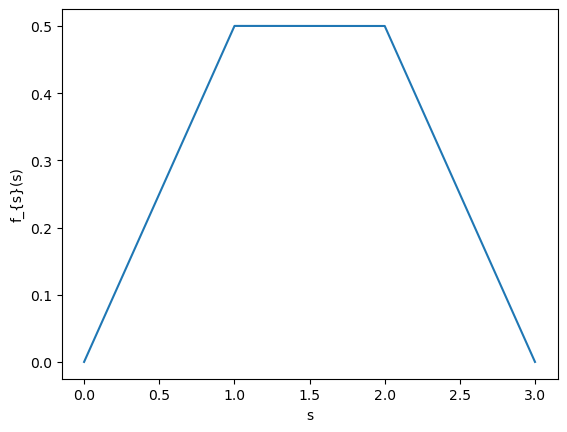
\includegraphics[width=10cm]{homework/homework_4/immages/q_1_!.png}
\item directly implementing my formula yielded the first plot
\item 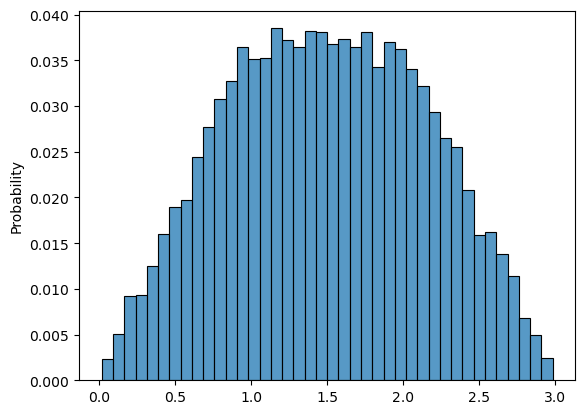
\includegraphics[width=10cm]{homework/homework_4/immages/q_1_2.png}
\item simulation gave me the second plot
\item it is encouraging that they agree
\end{itemize}



\newpage
\item (Confidence intervals) The following are $1-\alpha$ confidence intervals for a certain quantity $\mu$, estimated using the sample mean of the observed data. \vspace{0.2cm}\\
\begin{tabular}{>{\centering\arraybackslash}m{0.05\linewidth} >{\centering\arraybackslash}m{0.9\linewidth} }
 A  &
  \includegraphics[width=0.7\linewidth]{./hw4/figs/confidence_intervals_exam_20}   \\
  B &
  \includegraphics[width=0.7\linewidth]{./hw4/figs/confidence_intervals_exam_500} 
\end{tabular}
\begin{enumerate}
\item Estimate $\alpha$.
\begin{itemize}
\color{blue}
    \item each of the fugues has approx 40 confidence intervals and about 4 fail to capture the parameter in each. so i would estimate $\alpha=.1$.
\end{itemize}
\item In each scenario choose whether you think $X=A$ and $Y=B$, or $X=B$ and $Y=A$. \begin{itemize}
\item In plot X the confidence intervals are based on the central limit theorem. In plot Y they are built using Chebyshev's inequality (everything else is the same).


\item In plot X the confidence intervals are built using more data than in plot Y (everything else is the same).
\item In plot X the data are sampled from a distribution that has higher variance than plot Y (everything else is the same).
\begin{itemize}
     \color{blue}
    \item in the first case i think X=B and Y=A. this makes sense since the central limit theorem gives us a tighter bound on our uncertainty than Chebyshev's inequality so confidence intervals fit using that estimation would be smaller
    \item in the second case i think X=B and Y=A. this makes sense since assuming the assumptions of the central limit theorem are met, more data would result in lower standard error and thus tighter confidence intervals 
    \item in the first case i think X=A and Y=B. this makes sense as the width of confidence intervals are still determined by the variance of the underlying population we are trying to estimate so if there is more variance it is reasonable that we would have wider confidence intervals holding all else equal
\end{itemize}


\end{itemize}
\end{enumerate}
\newpage
\item (Cholesterol) We want to determine whether men have higher cholesterol than women in a certain population. We pick $200$ men and $100$ women independently at random with replacement from the population and compute their average cholesterol levels.  

\begin{enumerate}
\item Let $\sigma_{\text{men}}$ and $\sigma_{\text{women}}$ denote the standard deviations of the cholesterol level for the men and women in the population respectively. What is the standard error of the difference between the average cholesterol levels computed from our data?
\begin{itemize}
\color{blue}
    \item we are told that we are independently and randomly from a population. thus as our goal is to understand the difference between men and woman within our population, we can think of our large sample as made up two independent sub samples from the sub-populations of men and woman respectively
    \item further we know in both cases we have a frailly large number of samples (at least 100)
    \item thus i would argue that the assumptions of the central limit theorem are met. and it is reasonable to model the average cholesterol on our samples as two Gaussian random variables with mean's equal to there sub population mean and standard error equal to $\frac{\sigma_{men}}{\sqrt{200}}$,$\frac{\sigma_{women}}{\sqrt{100}}$ respectively
    \item so call the average cholesterol in our sample of men $\Tilde{m}_{men}=\frac{1}{n}\Sigma_{i=1}^{n}\Tilde{x}_{men}_{i}$ where $\Tilde{x}_{men}_{i}$ is the cholesterol of the ith man in our sample and call the average cholesterol in our sample of woman $\Tilde{m}_{women}=\frac{1}{n}\Sigma_{i=1}^{n}\Tilde{x}_{women}_{i}$ where $\Tilde{x}_{women}_{i}$ is the cholesterol of the ith woman in our sample
    \item thus we can writ the difference between average cholesterol in men and women in our sample as $\Tilde{d}=\Tilde{m}_{men}-\Tilde{m}_{women}$
    \item as our samples were taken independently we know  $var(\Tilde{d})=var(\Tilde{m}_{men})+var(\Tilde{m}_{women})-2cov(\Tilde{m}_{men},\Tilde{m}_{women})=var(\Tilde{m}_{men})+var(\Tilde{m}_{women})=\frac{\sigma_{men}^2}{200}$+$\frac{\sigma_{women}^2}{100}$
    \item and thus the standard deviation of our estimator is $se(\Tilde{d})=\frac{\sigma_{men}}{\sqrt{200}}+\frac{\sigma_{women}}{10}$
\end{itemize}


\item The average cholesterol levels we observe are 200 for the men and 180 for the women. Assuming $\sigma_{\text{men}} = \sigma_{\text{women}}=10$, compute a 95\% confidence interval for the difference between the mean cholesterol level for men and women in the population using the central limit theorem. %(Use the fact that $\Phi(1.95)=0.025$, where $\Phi$ is the cdf of a standard Gaussian.)
\begin{itemize}
    \color{blue}
    \item we can in general write a $1-\alpha$ confidence interval as $\Tilde{\mathcal{I}}_{1-\alpha}=[\Tilde{m}-c_{\alpha}se(m),\Tilde{m}+c_{\alpha}se(m)]$
    \item so all we really need is to get the parts 
    \begin{itemize}
        \item as we have $\1-\alpha=.95$ we know $c_{\alpha}=1.96$
        \item we defined our estimator of the difference between the average cholesterol level of men and women as $\Tilde{d}=\Tilde{m}_{men}-\Tilde{m}_{women}$ and we are given values for this estimate thus  $\Tilde{d}=\Tilde{m}_{men}-\Tilde{m}_{women}=200-180=20$ 
        \item we solved for the standard error above as  $se(\Tilde{d})=\frac{\sigma_{men}}{\sqrt{200}}+\frac{\sigma_{women}}{10}$ which we can evaluate here as  $se(\Tilde{d})=\frac{10}{\sqrt{200}}+\frac{10}{10}=1.707$
    \end{itemize}
    \item thus we can construct a 95\% confidence interval for the difference in average cholesterol between men and woman from our estimate as $\Tilde{\mathcal{I}}_{95}=[20-(1.96)*(1.707),20+(1.96)*(1.707)]=[16.65,23.34]$
\end{itemize}


\end{enumerate}
\newpage
\item (Blood pressure cont. HW3)
The table in \texttt{cardio.csv} records the systolic blood pressure (\textit{``ap\_hi"}) of a cohort of patients. In HW3, we compared the Chebyshev bound with the probability that \textit{ap\_hi} deviates from the corresponding population mean via Monte Carlo simulations.

\begin{enumerate}
    \item  Try to use the central limit theorem to approximate the probability. Plot the new approximation in the same plot as HW3 Q4.
    \begin{itemize}
        \color{blue}
        \item 
        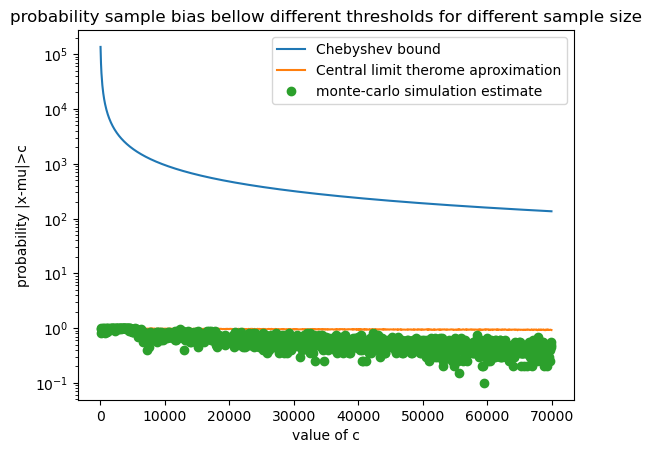
\includegraphics[width=10cm]{homework/homework_3/immages/hw_4_1.png}
        \item we can see that for a fixed $\alpha$ (in this case .5) the central limit theorem establishes a much more tight bound on the probability of our sample mean deviating then Chebyshev bound 
    \end{itemize}

    
    \item Compute approximate $1-\alpha$ confidence intervals of the sample mean for 50 batches of $n$ samples for $n \in \keys{50, 100}$ and $\alpha \in \keys{0.05, 0.1, 0.5}$. For each $n$ and $\alpha$, plot the confidence intervals together with the population mean of the full dataset and count the number of times that the population mean does not fall in the confidence interval. How do the values of $n$ and $\alpha$ influence (1) the length of the intervals and (2) the probability that the population mean belongs to the interval?
    \begin{itemize}
        \color{blue}
        \item the charts are bellow this response. 
        \item 1. $1-\alpha$ is the portion of confidence intervals over many samples that contain the true population parameter, so as $\alpha$ rises the confidence interval gets more narrow. Other things being equal as the number of samples rise our variance of the sample mean should fall so the width of the interval is reducing in n
        \item 2. $1-\alpha$ is the portion of confidence intervals over many samples that contain the true population parameter, so as $\alpha$ rises the chance that our population parameter is in the confidence interval falls. As n goes up we are basing our estimator on more data so the likelihood of the estimator contains the true population parameter is rising in n. 
        \item 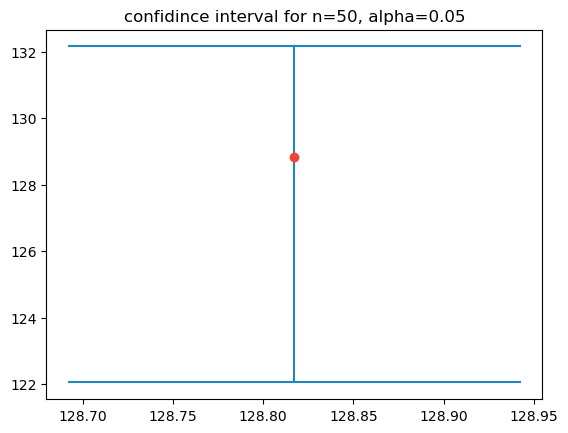
\includegraphics[width=10cm]{homework/homework_3/immages/hw_4_2.png}
        \item 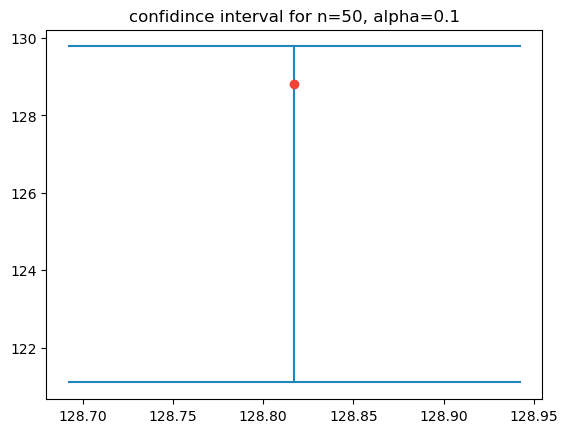
\includegraphics[width=10cm]{homework/homework_3/immages/hw_4_3.png}
        \item 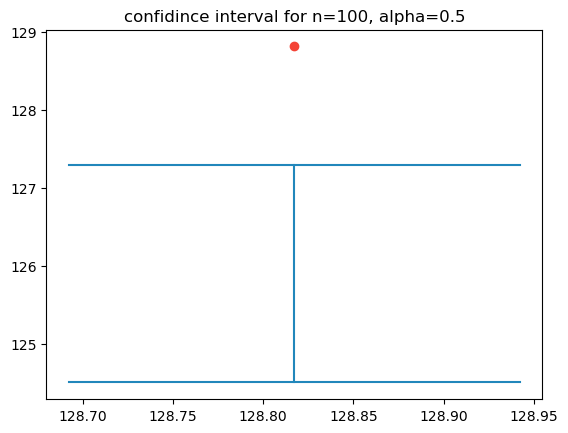
\includegraphics[width=10cm]{homework/homework_3/immages/hw_4_4.png}
        \item 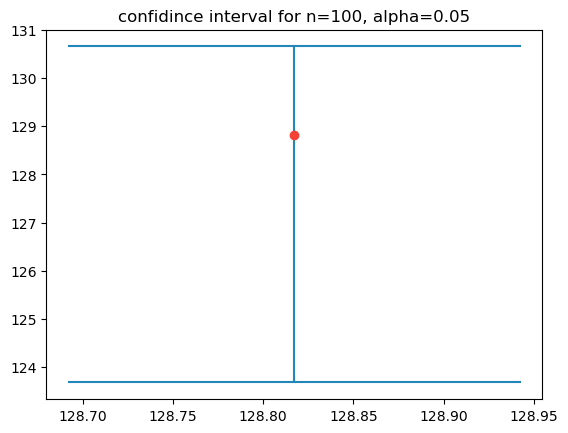
\includegraphics[width=10cm]{homework/homework_3/immages/hw_4_5.png}
        \item 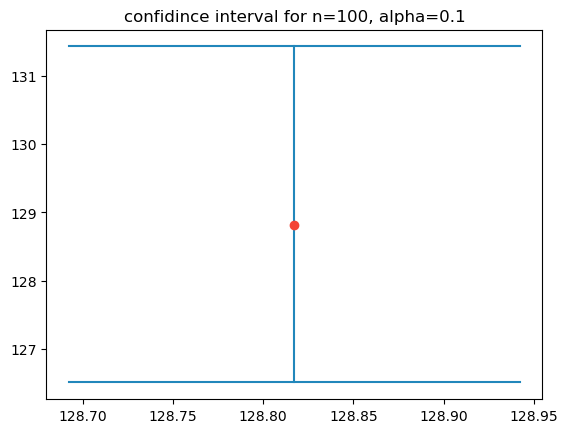
\includegraphics[width=10cm]{homework/homework_3/immages/hw_4_6.png}
        \item 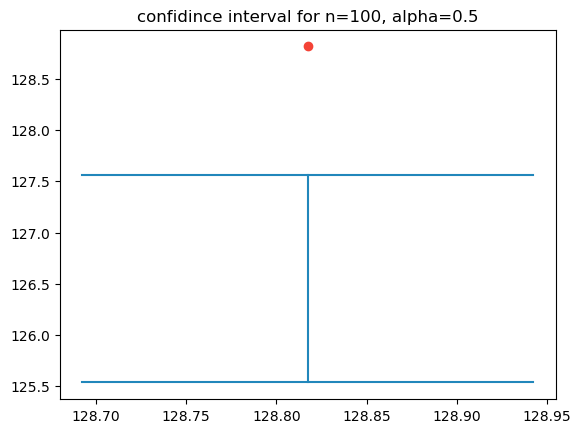
\includegraphics[width=10cm]{homework/homework_3/immages/hw_4_7.png}
    \end{itemize}
\end{enumerate}


\end{enumerate}
\end{document}
